%%%%%%%%%%%%%%%%%%%%%%%%%%%%%%%%%%%%%%%%%%%%%%%%%%%%%%
% A Beamer template for University of Wollongong     %
% Based on THU beamer theme                          %
% Author: Qiuyu Lu                                   %
% Date: July 2024                                    %
% LPPL Licensed.                                     %
%%%%%%%%%%%%%%%%%%%%%%%%%%%%%%%%%%%%%%%%%%%%%%%%%%%%%%
% Customized for Sharif University of Technology     %
%%%%%%%%%%%%%%%%%%%%%%%%%%%%%%%%%%%%%%%%%%%%%%%%%%%%%%


\documentclass[serif, aspectratio=169]{beamer}
%\documentclass[serif]{beamer}  % for 4:3 ratio
\usepackage[T1]{fontenc} 
\usepackage{fourier} % see "http://faq.ktug.org/wiki/uploads/MathFonts.pdf" for other options
\usepackage{hyperref}
\usepackage{latexsym,amsmath,xcolor,multicol,booktabs,calligra}
\usepackage{graphicx,pstricks,listings,stackengine}
\usepackage{lipsum}
\usepackage{tikz}
\usetikzlibrary{shapes.geometric} % Add this to include ellipse shapes
\usepackage{amsmath}
\usepackage{pgfplots}  % For plots
\usepackage{amsmath}   % For equations
\usepackage{array}     % For tables
\pgfplotsset{compat=1.16}

% \usetikzlibrary{positioning}


\author{Ali Sharifi-Zarchi}
\title{Machine Learning (CE 40717)}
\subtitle{Fall 2024}
\institute{
    CE Department \\
    Sharif University of Technology
}
%\date{\small \today}
% \usepackage{UoWstyle}
\usepackage{SUTstyle}

% defs
\def\cmd#1{\texttt{\color{red}\footnotesize $\backslash$#1}}
\def\env#1{\texttt{\color{blue}\footnotesize #1}}
\definecolor{deepblue}{rgb}{0,0,0.5}
\definecolor{deepred}{RGB}{153,0,0}
\definecolor{deepgreen}{rgb}{0,0.5,0}
\definecolor{halfgray}{gray}{0.55}

\lstset{
    basicstyle=\ttfamily\small,
    keywordstyle=\bfseries\color{deepblue},
    emphstyle=\ttfamily\color{deepred},    % Custom highlighting style
    stringstyle=\color{deepgreen},
    numbers=left,
    numberstyle=\small\color{halfgray},
    rulesepcolor=\color{red!20!green!20!blue!20},
    frame=shadowbox,
}

\begin{document}

\begin{frame}
    \titlepage
    \vspace*{-0.6cm}
    \begin{figure}[htpb]
        \begin{center}
            
\includegraphics[keepaspectratio, scale=0.25]{pic/sharif-main-logo.png}
        \end{center}
    \end{figure}
\end{frame}

\begin{frame}    
\tableofcontents[sectionstyle=show,
subsectionstyle=show/shaded/hide,
subsubsectionstyle=show/shaded/hide]
\end{frame}

% ============================ Introduction ============================ 
\section{Introduction}

\begin{frame}{Self-Supervised Learning}
    \begin{picture}(0,0)
            \put(200,-150){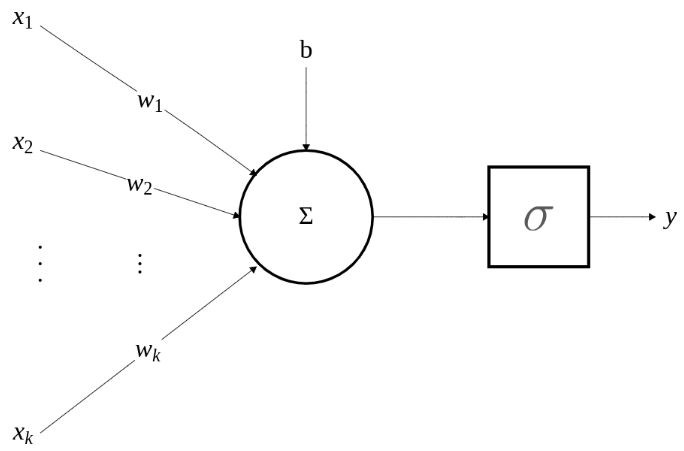
\includegraphics[width=7cm]{pic/1/neuron.png}} % Adjust path and size
    \end{picture}
     “the dark matter of intelligence” \footnote{\url{https://ai.meta.com/blog/self-supervised-learning-the-dark-matter-of-intelligence/}}
    \begin{itemize}
        \item $\{x_1, x_2, \dots, x_k\}$ : input features
        \item $\{w_1, w_2, \dots, w_k\}$ : feature weights
        \item $b$ : bias term
        \item $\sigma(\cdot)$ : activation function
        \item $y$ : output of the neuron
    \end{itemize}
\end{frame}

\begin{frame}{Self-Supervised Learning}
    \begin{center}
        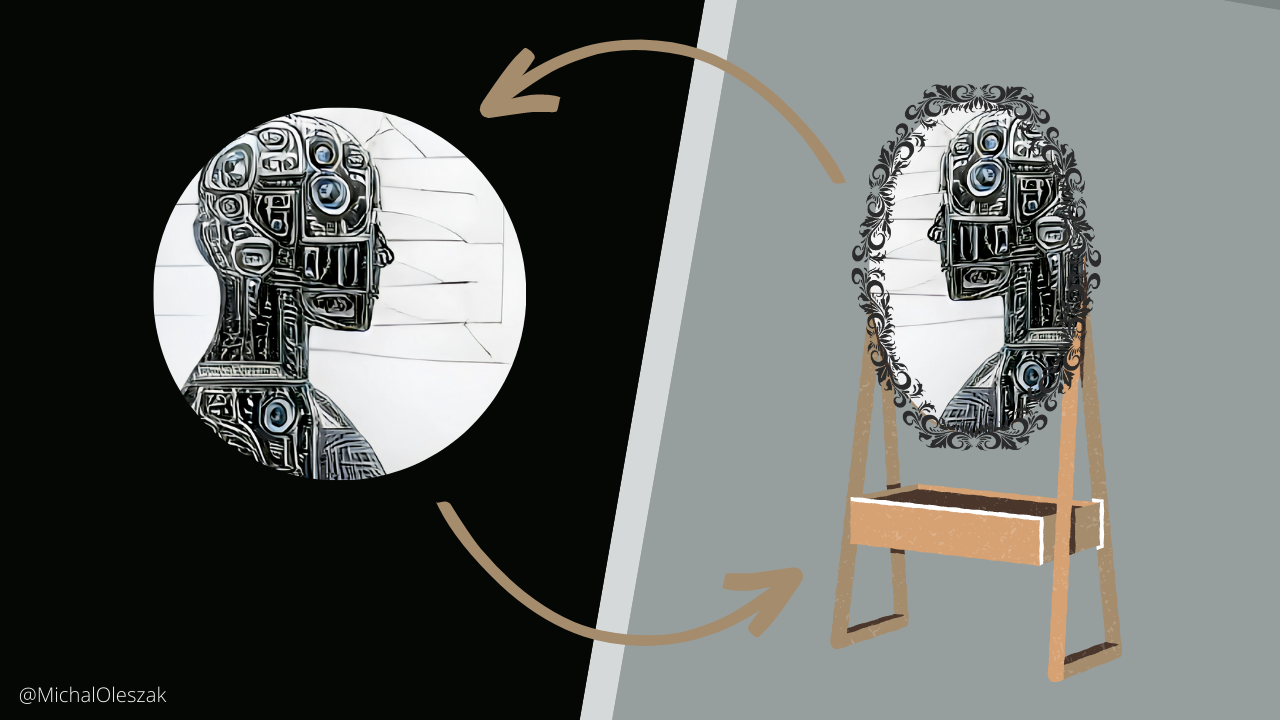
\includegraphics[width=0.6\textwidth]{pic/Intro.png} % Replace with the path to your image
        \\[1cm] % Adds space between image and quote
        \textit{“the dark matter of intelligence”}\footnote{\scriptsize \url{https://ai.meta.com/blog/self-supervised-learning-the-dark-matter-of-intelligence/}}
    \end{center}
\end{frame}

\begin{frame}{Why Neural Networks?}
    \begin{itemize}
        \item  Self-supervised learning defines a "pretext" task based on unlabeled inputs to produce descriptive and intelligible representations [Hastie et al., 2009, Goodfellow et al., 2016]
        \begin{itemize}
            \item Learn with supervised learning objectives, e.g., classification, regression.
	\item Labels of these pretext tasks are generated \textit{automatically}
	\item Can be used in other downstream tasks.
        \end{itemize}
    \end{itemize}
\end{frame}


\begin{frame}[t]{Example Workflow}
    
    \begin{itemize}
\item Training objective: predicting the context surrounding a word
\item encourages the model to capture relationships among words
\item The same SSL model representations can be used across a range
 of downstream tasks. e.g.
        \begin{itemize}
	\item translating text across languages
	\item summarizing
	\item generating text
        \end{itemize}
    \end{itemize}

\end{frame}

\begin{frame}[t]{Motivation}
  
    \begin{itemize}
        \item Problem: Supervised Learning is Expensive!
            \begin{itemize}
        \item Labeling data is costly
\item SSL: Use signals that can be created automatically from data.
    \end{itemize}
\item Labled data is harder to find. There is much more unlabled data.
\item Supervised Learning is not how "we" learn
  \begin{itemize}
 \item Babies don’t get supervision for everything they see!

     \end{itemize}

    \end{itemize}

\end{frame}



\begin{frame}[t]{Comparison}
Methods that learn from data without annotations.
    \begin{itemize}
        
\item \textbf{ Unsupervised Learning}: Model isn’t told what to predict. Older 
terminology, not used as much today.
 \item \textbf{ Self-Supervised Learning}: Model is trained to predict some naturally
occurring signal in the raw data rather than human annotations.
 \item \textbf{  Semi-Supervised Learning}: Train jointly with some labeled data and (a lot)
 of unlabeled data
    \end{itemize}
\end{frame}

\iffalse
\begin{frame}{Comparison of Learning Paradigms}

    \begin{center}
        \begin{tabular}{|c|c|c|c|}
            \hline
            \textbf{Aspect} & \textbf{Supervised} & \textbf{Unsupervised} & \textbf{Self-Supervised} \\ \hline
            \textbf{Data Labels} & Required & Not Required & Pseudo-Labels \\ \hline
            \textbf{Goal} & Predict labels & Find patterns/structure & Learn representations \\ \hline
            \textbf{Example Tasks} & Classification, Regression & Clustering, Dimensionality Reduction & Pretraining for downstream tasks \\ \hline
            \textbf{Examples} & Image classification, spam detection & K-means, PCA & BERT, SimCLR \\ \hline
            \textbf{Strengths} & Accurate when data is labeled & Useful when labels are scarce & Leverages unlabeled data effectively \\ \hline
            \textbf{Weaknesses} & Requires labeled data & Limited to pattern discovery & Requires complex pseudo-label generation \\ \hline
        \end{tabular}
    \end{center}
\end{frame}
\fi

\iffalse
\begin{frame}{Comparison of Learning Paradigms}
(COMMENTED SLIDE)
    \begin{center}
        \begin{tabular}{l l l l}
            \textbf{Aspect} & \textbf{Supervised} & \textbf{Unsupervised} & \textbf{Self-Supervised} \\[0.3cm]
            \hline \\[-0.3cm]
            \textbf{Data Labels} & Required & Not Required & Pseudo-Labels \\[0.3cm]
            \textbf{Goal} & Predict labels & Find patterns/structure & Learn representations \\[0.3cm]
            \textbf{Example Tasks} & Classification, Regression & Clustering, Dimensionality Reduction & Pretraining for downstream tasks \\[0.3cm]
            \textbf{Examples} & Image classification, spam detection & K-means, PCA & BERT, SimCLR \\[0.3cm]
            \textbf{Strengths} & Accurate when data is labeled & Useful when labels are scarce & Leverages unlabeled data effectively \\[0.3cm]
            \textbf{Weaknesses} & Requires labeled data & Limited to pattern discovery & Requires complex pseudo-label generation \\[0.3cm]
        \end{tabular}
    \end{center}
\end{frame}
\fi

%


\begin{frame}{Evaluation}
    \begin{itemize}
       \item We usually don’t care about the performance of the self-supervised learning task, e.g., we don’t care if the model learns to predict image 
rotation perfectly.
 \item Evaluate the learned feature encoders on downstream target tasks

    \end{itemize}
\end{frame}

\begin{frame}{Evaluation Cont.}
        
     \begin{flushleft}
           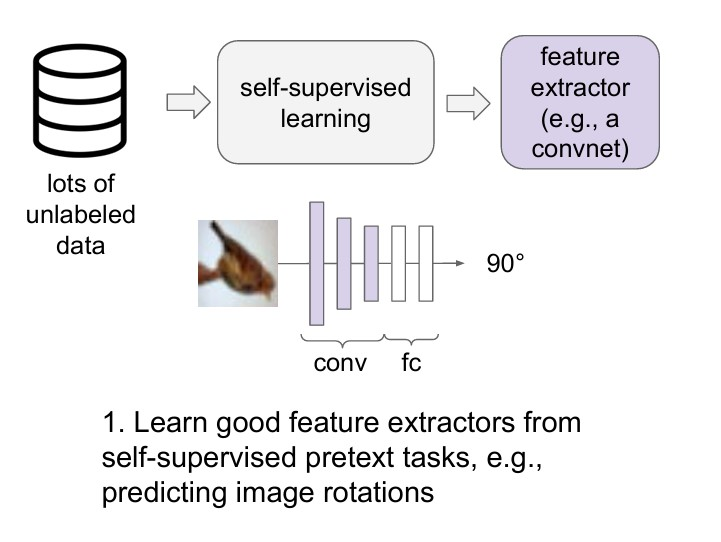
\includegraphics[keepaspectratio, scale=0.5]{pic/Evaluation-1.jpg}
\end{flushleft}
  
\end{frame}


\begin{frame}{Evaluation Cont.}
        \begin{figure}[htpb]
   
           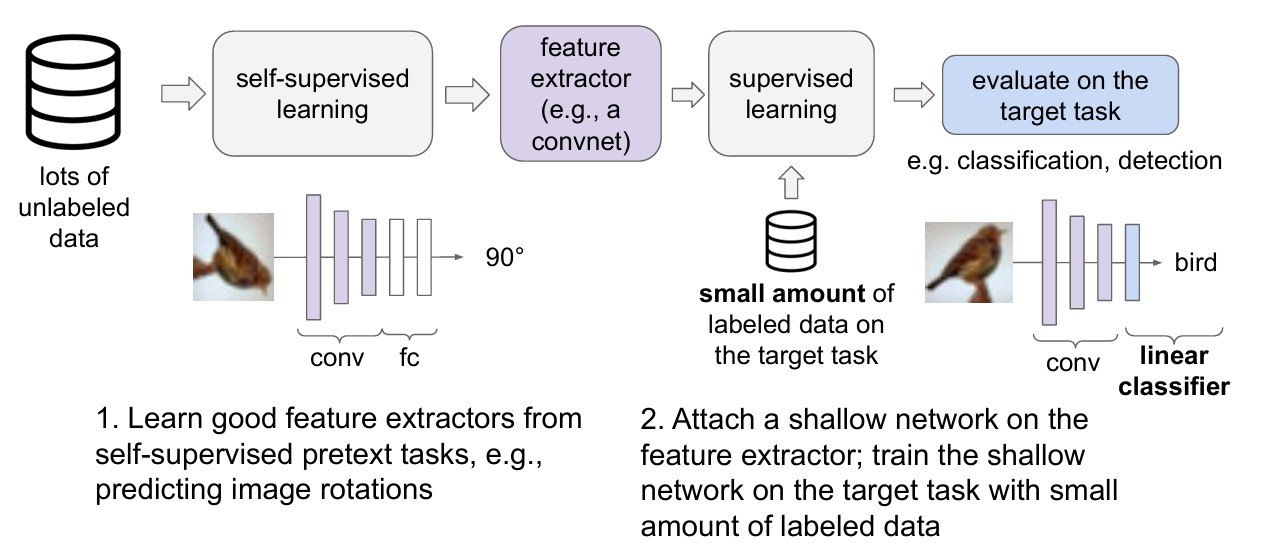
\includegraphics[keepaspectratio, scale=0.5]{pic/Evaluation-2.jpg}

    \end{figure}
\end{frame}


\begin{frame}{Example}
      \begin{itemize}
 \item Pretext task: predict rotations
\item  Hypothesis: a model could recognize the correct rotation of an object 
only if it has the “visual commonsense” of what the object should look 
like unperturbed.
\item The model learns to 
predict which rotation 
is applied (4-way 
classification)
\item (This slide will be ellaborated on and expanded with diagrams)

  \end{itemize}
\end{frame}

\section{Multimodal and CLIP}


\begin{frame}{Idea}
     
 \begin{itemize}
 \item    Many papers would pretrain on (unlabeled) ImageNet, then evaluate on ImageNet!
 \item  Don’t learn from isolated images -- take images together with some \textbf{context}
\item Video: Image together with adjacent video frames
 \item Sound: Image with audio track from video
 \item 3D: Image with depth map or point cloud
\item  \color{purple}{ Language: Image with natural-language text }

  \end{itemize}
\end{frame}

\begin{frame}{Why Language ?}
    \begin{columns}
        \begin{column}{0.5\textwidth}
            \begin{itemize}
          \item      Semantic density: Just a few 
words give rich information
 \item  Universality: Language 
can describe any concept
\item  Scalability: Non-experts 
can easily caption images;
 data can also be collected 
from the web at scale
 
            \end{itemize}
        \end{column}
        \begin{column}{0.5\textwidth}
            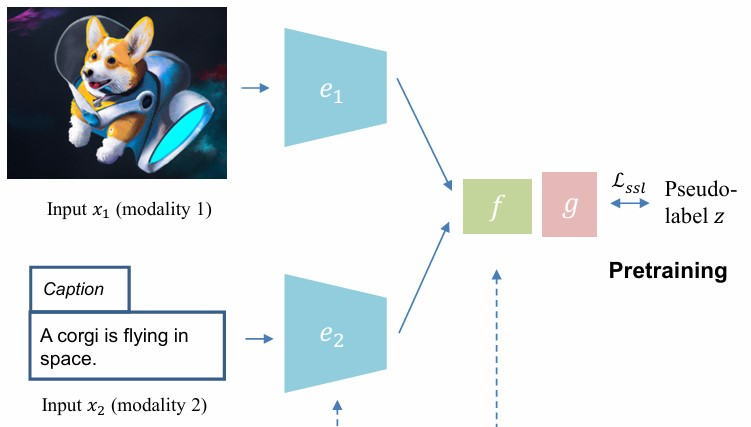
\includegraphics[width=\textwidth]{pic/MultiModal-1.jpg} \\
            \begin{center}
            {\scriptsize Adapted from} % \href{https://sefiks.com/2020/02/02/dance-moves-of-deep-learning-activation-functions/}{Sefiks}}
            \end{center}
        \end{column}
    \end{columns}
\end{frame}



\begin{frame}{Common Components}
    \begin{itemize}
        \item Dataset :
\begin{itemize}
\item supervised:  $D_m = \{ (x_1^1, \cdots, x_M^1, y^1), \cdots, (x_1^n, \cdots, x_M^n, y^n)  \}$
\item self-supervised:  $D_m = \{ (x_1^1, \cdots, x_M^1), \cdots, (x_1^n, \cdots, x_M^n)  \}$
\end{itemize}
\item The psudo-label or signal generated for SSL can be denoted as $z = P(x_1,\cdot,x_M)$.

        \item Modality Encoder(s): $c = e_k(x_k^i; \theta_k)$ for each modality $k$.
	\item Fusion Module: $f_\psi$ to integrate the encoded information of different modalities
	\item Pretext task head (like a predictive head) : $g_\gamma$ and some SSL loss $\mathcal{L}_{SSL}$

    \end{itemize}
\end{frame}


\begin{frame}{Architectures}
  \begin{itemize}
\item There many veriations and structures
  \end{itemize}
 \begin{minipage}{0.48\textwidth} % Adjust the width as needed
        \begin{figure}
	\centering
        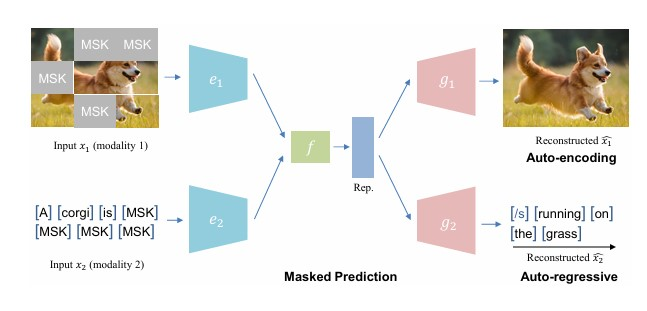
\includegraphics[width=\textwidth]{pic/SSL-MM-var1.jpg} % Replace with your image path
        \caption{Figure 1 masked prediction frameworks} % Optional
   \end{figure}
    \end{minipage} \hfill % Add some space between the two images
    \begin{minipage}{0.48\textwidth}
   \begin{figure}
        \centering
        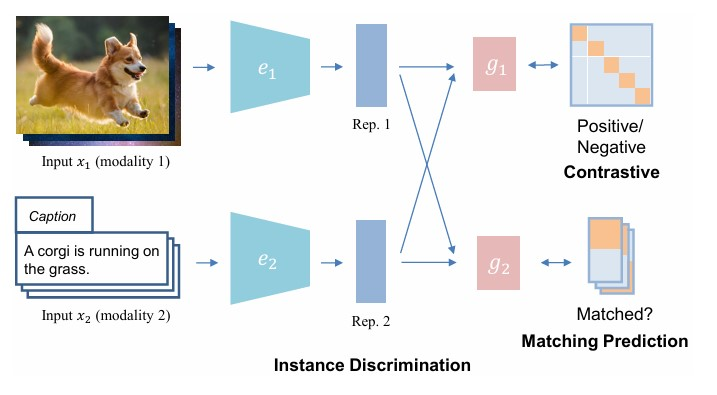
\includegraphics[width=\textwidth]{pic/SSL-MM-var2.jpg} % Replace with your image path
        \caption{Figure 2 instance discrimination objectives} % Optional
   \end{figure}
    \end{minipage}
\end{frame}

\begin{frame}{Contrastive Loss}
\begin{itemize}
\item (Put Contrastive Loss Slides here)
\end{itemize}
\end{frame}

\begin{frame}{CLIP}
\begin{itemize}
\item Connecting text and images
\item Contrastive Language–Image Pre-training
\item CLIP $\implies$ a shared representation(embedding) between two modalities (text and images) by training on a large dataset of image-text pairs.
\end{itemize}
\end{frame}

\begin{frame}{CLIP Cont.}
\begin{itemize}
\item Image Encoder: a Vision Transformer (ViT) or a ResNet.
\item Text Encoder: A Transformer model 
\end{itemize}
\begin{figure}[hb]
        \begin{center}
            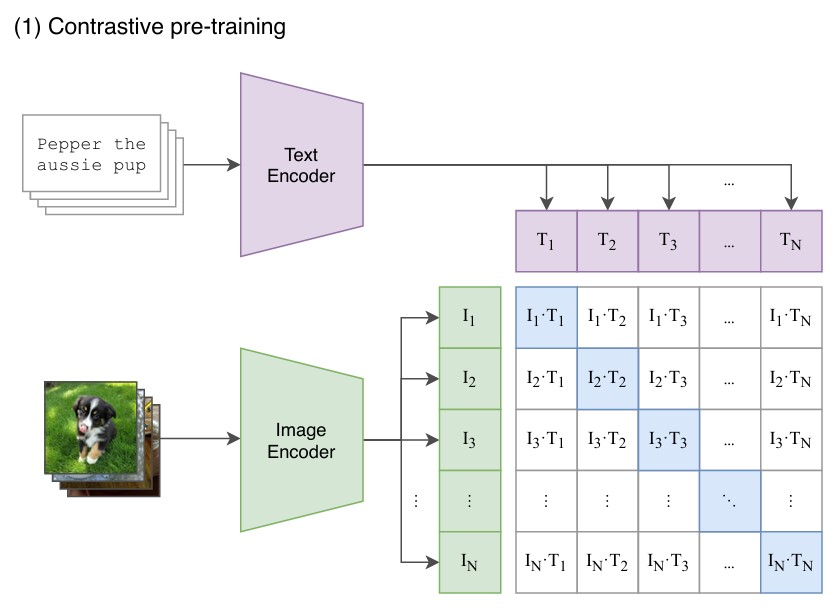
\includegraphics[keepaspectratio, scale=0.5]{pic/clip-overview.jpg}
        \end{center}
    \end{figure}
\end{frame}


\begin{frame}{CLIP Goals}
\begin{itemize}
\item CLIP was designed to mitigate a number of major problems:
\item Costly datasets: Deep learning needs a lot of data, manually labeled datasets are expensive to construct.
\begin{itemize}
\item CLIP learns from text–image pairs that are already publicly available on the internet
\end{itemize}
\item Narrow: An ImageNet model excels at predicting the 1000 ImageNet categories but requires additional data and fine-tuning for other tasks. 

\begin{itemize}
\item CLIP can be adapted to perform a wide variety of visual classification tasks without needing additional training examples. 
\end{itemize}
\end{itemize}

\end{frame}


\begin{frame}{Zero-Shot Classification}
\begin{itemize}
\item (Put Zero-Shot and Applications Slides here)
\end{itemize}
\end{frame}

\section{References}

\begin{frame}{Contributions}
\textbf{These slides are authored by:}
    \begin{itemize}
        \item Hooman Zolfaghari
    \end{itemize}
    
\end{frame}


\begin{frame}[allowframebreaks]
   \bibliographystyle{ieeetr} % Place the style before bibliography
   \bibliography{ref.bib} % Point to your .bib file
   \nocite{*} % Include all references even if not cited
\end{frame}


\end{document}